%\documentclass[draft]{beamer}
\documentclass{beamer}
\usetheme{Warsaw}
\usecolortheme{wolverine}
\usepackage{graphicx}
\usepackage{amsmath}
\usepackage{amsfonts}
\usepackage{amssymb}
\usepackage{amsthm}
\DeclareMathOperator{\Li}{Li}

\newcommand{\mysection}[2]{\section{\S#1. #2}%
\begin{frame}{}
\vfill
\begin{center}
\hrulefill
\vfill
\Huge\sc \S#1. #2
\vfill
\hrulefill
\end{center}
\vfill
\end{frame}}

\title{Writing a book with Barry Mazur}
\subtitle{``Prime Numbers and the Riemann Hypothesis''}
\author[W.\thinspace{}Stein]{William Stein}
\date[Mazur 80]{June 4, 2018 at Harvard University}
\institute[SageMath, Inc. \& UW]{SageMath, Inc. and University of Washington}


\begin{document}

\begin{frame}
  \titlepage
\end{frame}

\begin{frame}{Abstract}
  \begin{abstract}
    In 2004, Barry Mazur and I started a decade project to write the
    book ``Prime Numbers and the Riemann Hypothesis''.
    This talk is about
    what's in the book and why, and some aspects
    of production of the book.
  \end{abstract}
\end{frame}

\begin{frame}{Prelude: collaborate with great co-authors!}

Writing John Tate's {\em Galois Cohomology} notes for PCMI 1999...

\vfill

\begin{block}{}
{\em
``Everybody is so jealous of you getting
to talk with John Tate!''}\\
 -- David Savitt
  \end{block}

\vfill

If you ever get the chance
to write something with someone incredible,
{\bf\em take it!!}

\vfill

(I next wrote a long paper with Ken Ribet from that same PCMI.)

\end{frame}


\begin{frame}{Overview}
  \tableofcontents
\end{frame}

% todo: add a picture for each section start.
% this one -- picture of Barry giving a talk (e.g., screen capture from MSRI lecture)
\mysection{1}{Barry's Public Lecture}

\begin{frame}{Clay Math Institute public lecture (MIT, May 3, 2005)}
\begin{center}
  \href{http://www.claymath.org/library/public\_lectures/mazur\_riemann\_hypothesis.pdf}{\small\underline{``Are there still unsolved problems about the numbers 1, 2, 3, 4, ... ?''}}
\end{center}

  \vfill

  \begin{block}{Use primes to ``sell'' number theory to the general public}
    \begin{itemize}
      \item   Immediately accessible
      \item   Immediately interesting
      \item   Primes and how eratic they are
      \item   Cicada's every 13, 17 years...
      \item   Many examples of ``open, interesting questions''
      \item   People can immediately make computations of their \underline{own}
      \item   Barry got his father, who had done NO
            math, hooked on the Goldbach Conjecture, so thought
            primes would work.
    \end{itemize}
  \end{block}
\end{frame}

\begin{frame}{SageMath}
  \vfill
  \begin{center}
    
\includegraphics[width=.7\textwidth]{pics/sage-logo}
  \end{center}
  \vfill

  \begin{block}{2005: I started SageMath}
    I launched Sage a few months before this 2005 CMI public lecture.
    \begin{itemize}
      \item Sage is a {\bf free open source} alternative to Mathematica, Maple, Magma, and Matlab.
      \item Early Sage development motivated by this talk
            \begin{itemize}
              \item Linking Sage to Mathematica to compute $\Gamma$
              \item Early visualization functionality
              \item Prime enumeration
            \end{itemize}
    \end{itemize}
  \end{block}
\end{frame}

\begin{frame}{More about what was in Barry's public lecture...}
  \begin{block}{Barry's Public Lecture: Topics}
    \begin{itemize}
      \item Primes as atoms: factorization
      \item The largest known prime
      \item Enumerating primes: Sieve of Eratosthenes
      \item Twin primes
      \item Counting primes
      \item Gauss's Conjecture: The Prime Number Theorem
      \item Riemann: Fourier style smooth approximations $R_k(x)$ to $\pi(x)$
      \item Riemann's Harmonics: zeros of $\zeta(s)$
    \end{itemize}

  \end{block}

  \vfill
  \begin{center}
  \Large
  \emph{It worked!}
\end{center}



\end{frame}

\mysection{2}{Writing a Book}

\begin{frame}{``Let's write a book...'' -- Barry}
  \begin{block}{Could we turn this public lecture into a popular book?}

    \begin{itemize}
      \item Write something for a popular audience
      \item Small and readable
      \item Full of {\em mathematics}, not stories of people
      \item Profusely illustrated
      \item Meet for a few weeks in his country house and focus on this
    \end{itemize}
  \end{block}
\end{frame}


\begin{frame}{What kind of book?}

There are already 4 recent popular books on the Riemann Hypothesis.  Why write another?
\vfill

\begin{block}{Our general audience book could be unique}
  \begin{itemize}
    \item Motivated by deeply discussing the prime counting problem, and connecting it with our other research project on {\em the explicit formula}.
    \item Mostly math and not ``stories of people'' (other books on RH already do the stories well).
  \end{itemize}
  \end{block}
\end{frame}

\begin{frame}{What Sort of Book: Small, Medium or Large?}
  \begin{center}
    Like T.\thinspace{}C. MITS or like ON BULLSHIT?
    \vspace{1ex}

    
\includegraphics[height=.75\textheight]{pics/tc-mits}
    \hspace{2em}
    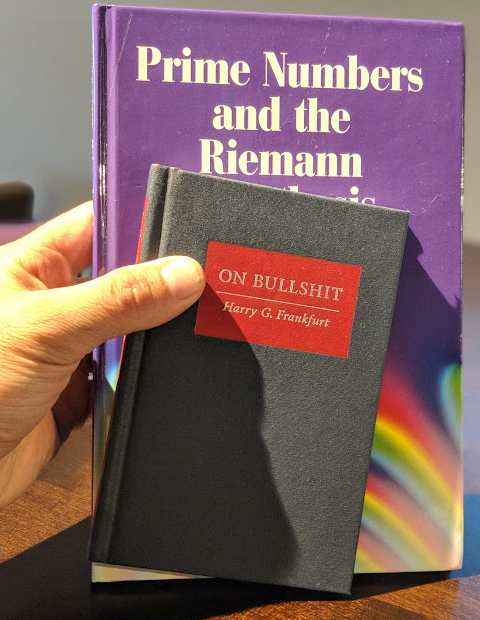
\includegraphics[height=.75\textheight]{pics/bullshit}
  \end{center}
\end{frame}


\begin{frame}{Our Approach}
  \begin{block}{}
    Go back 150+ years and explain what RH is more from the point of view of real classical Fourier analysis.
            \begin{itemize}
              \item Embrace a mid-19th century very $\mathbb{R}$eal perspective
              \item Leave $\mathbb{C}$omplex numbers to the very, very end
            \end{itemize}
  \end{block}
  \begin{center}
    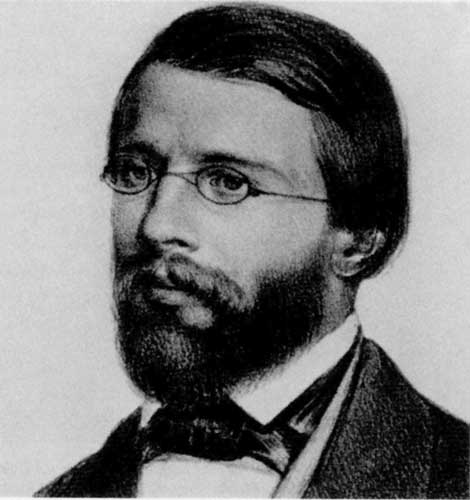
\includegraphics[height=.5\textheight]{pics/riemann}
  \end{center}

\end{frame}


\begin{frame}{Target Audience?}

\begin{block}{Who are we writing this book for?}
{\em Lovers of number theory}, who want to read about mathematics.
\vspace{.5in}

  \begin{itemize}
    \item \textbf{High school students?\footnote{Neither Barry nor I  graduated from high school...}} Tested at \href{https://wstein.org/edu/2007/simuw07/}{SIMUW 2007}.
    \item \textbf{Retired electrical engineers?}  Tested with original MIT talk, and  online materials we shared.
  \end{itemize}
\vspace{.5in}

\end{block}

\end{frame}


\begin{frame}{SageMath again}
\begin{block}{Computations with Sage drove the exposition}
  We used Sage to compute with prime numbers, zeros, etc., and generally to plot everything in the book.
  \begin{itemize}
    \item Numerous plots that are absolutely essential to the exposition, and in fact really drove it!
    \item Surprising to see so much with such little computation.
    \item Central hook of the book appears from computation:\\
    {\em ``Fourier transform links the discrete distribution at prime powers and the discrete distribution of zeros of $\zeta$.''}
    \item This is also what got us thinking about ``how explicit is the explicit formula?'' (another research project...)
  \end{itemize}
  \end{block}
\end{frame}


\begin{frame}{Collaborative \LaTeX{} via CoCalc}
  \begin{block}{How we wrote the book}
    \begin{itemize}
      \item Using CoCalc's \LaTeX{} editor.
            \begin{itemize}
              \item In a web browser...
              \item Both of us simultaneously editing the same file.
              \item Precise history of all changes
              \item Gives a sense of the collaborative spirit
              \item Plug: I just released a new version of the editor!
            \end{itemize}
      \item Rough PDF's of book on the web at every stage.
      \item \href{https://github.com/williamstein/rh}{GitHub tracking of changes}
      \item Sage computations run in the same place as editing book.
      \item Barry did very closely read and understand all the Sage code!
    \end{itemize}
  \end{block}
\end{frame}

\begin{frame}{Screenshot of CoCalc's Collaborative \LaTeX{} Editor}
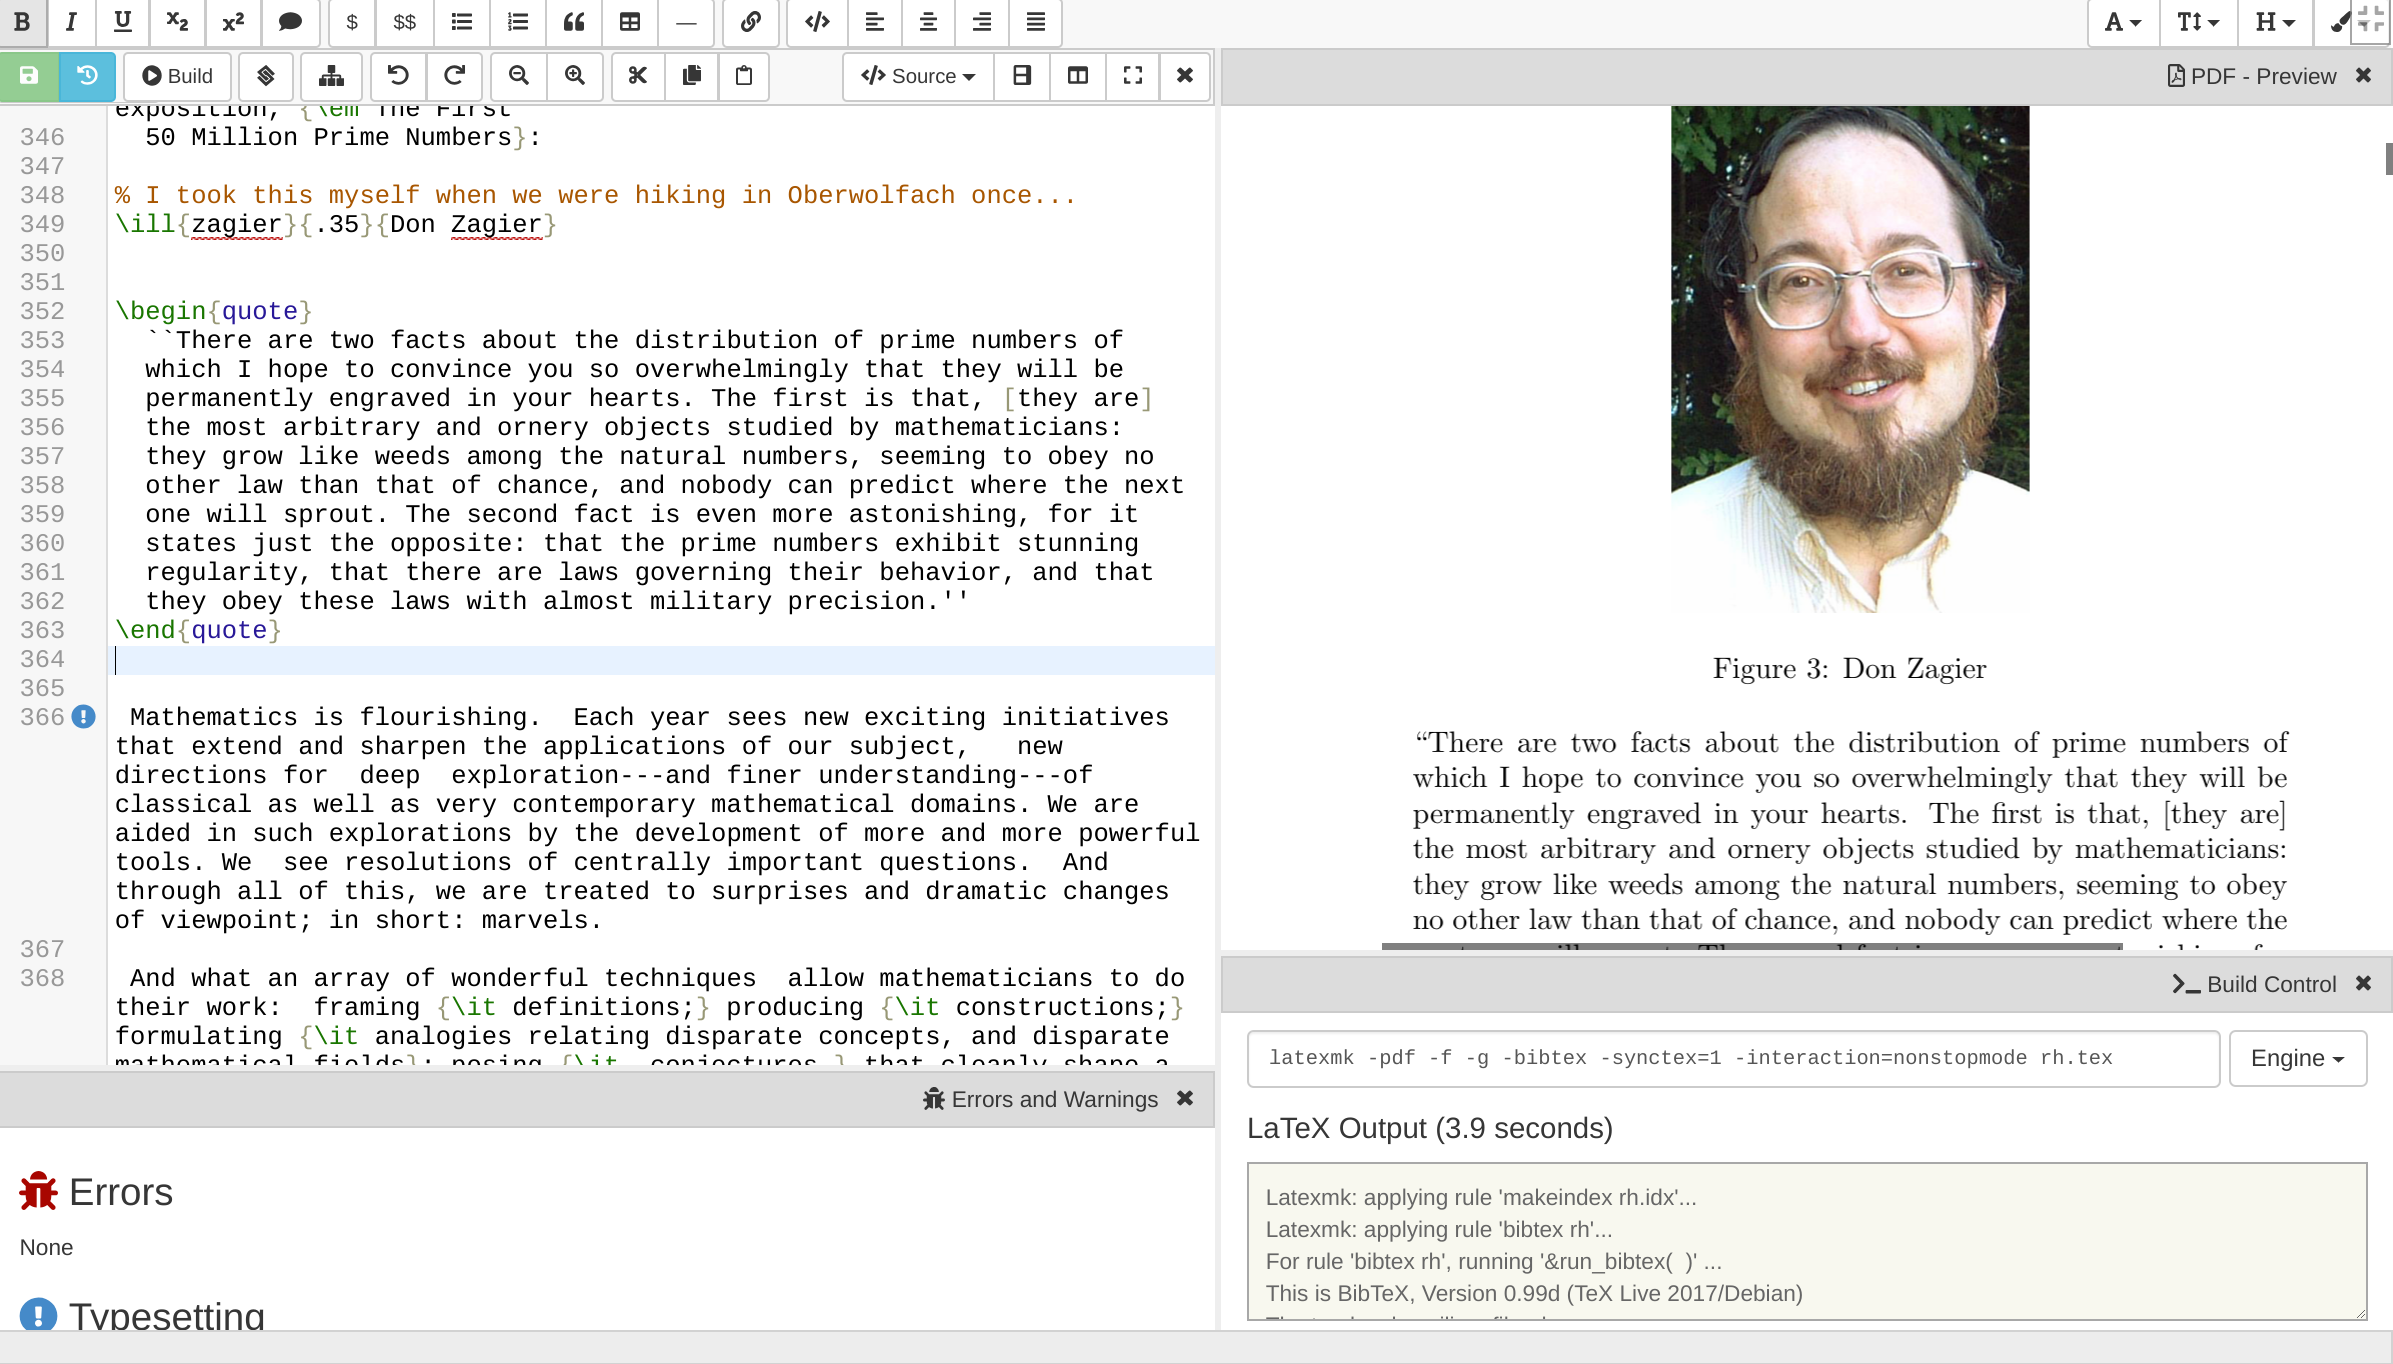
\includegraphics[width=\textwidth]{pics/cocalc-latex}
\end{frame}

\begin{frame}{}
\vfill
\begin{center}
\hrulefill
\vfill
\Huge\sc Here it is!
\vfill
\hrulefill
\end{center}
\vfill
\begin{center}
(in just a few slides)
\end{center}
\end{frame}


\begin{frame}{The Prime Counting Problem}
  Let $\pi(x)$ be the number of primes $\leq x$.\\
  {\bf Problem:} {\em Give a ``good approximation'' for $\pi(x)$.}
  \vfill

  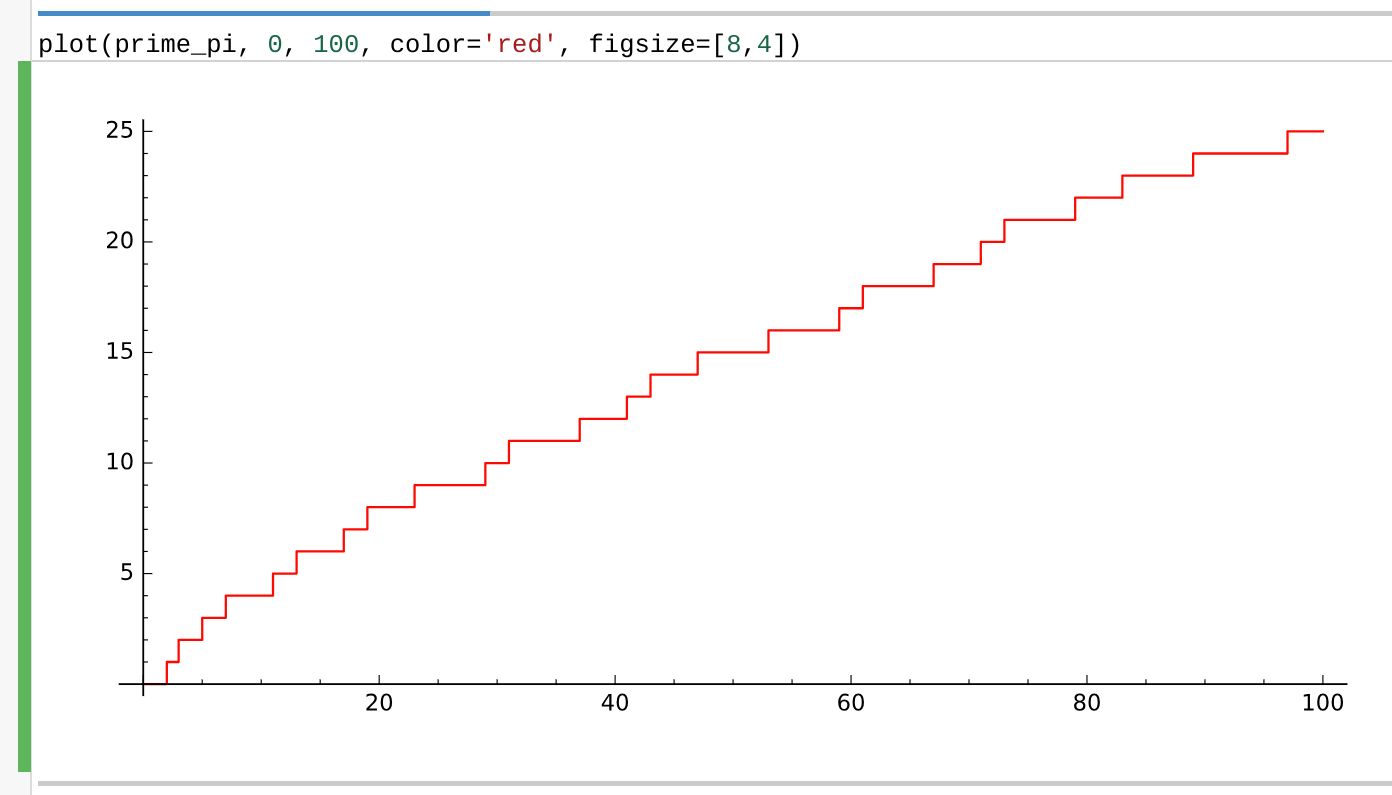
\includegraphics[width=.98\textwidth]{pics/prime-pi-100}

\end{frame}

\begin{frame}{The Prime Counting Problem}
  Let $\pi(x)$ be the number of primes $\leq x$.\\
  {\bf Problem:} {\em Give a ``good approximation'' for $\pi(x)$.}
  \vfill

  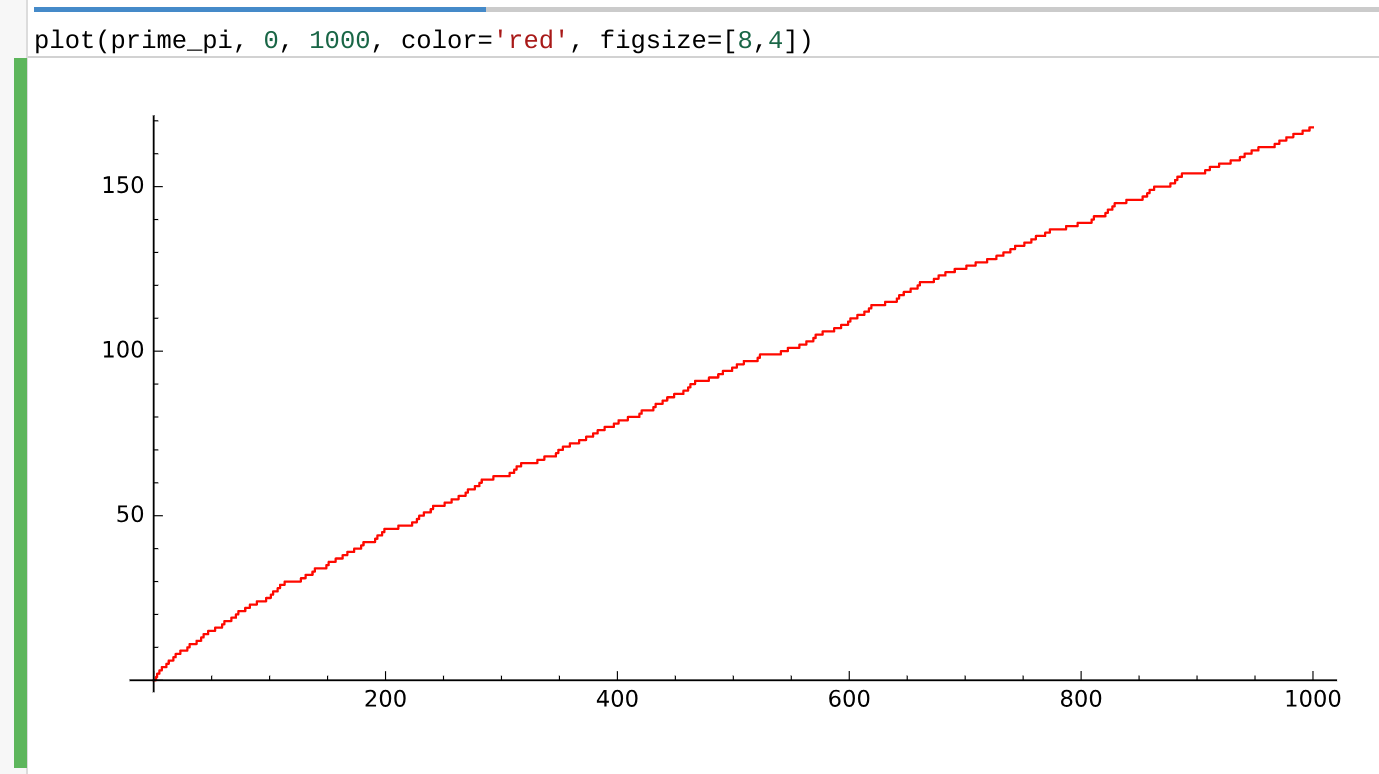
\includegraphics[width=.98\textwidth]{pics/prime-pi-1000}

\end{frame}

\begin{frame}{Focus on The Prime Counting Problem}
  Let $\pi(x)$ be the number of primes $\leq x$.\\
  {\bf Problem:} {\em Give a ``good approximation'' for $\pi(x)$.}
  \vfill

  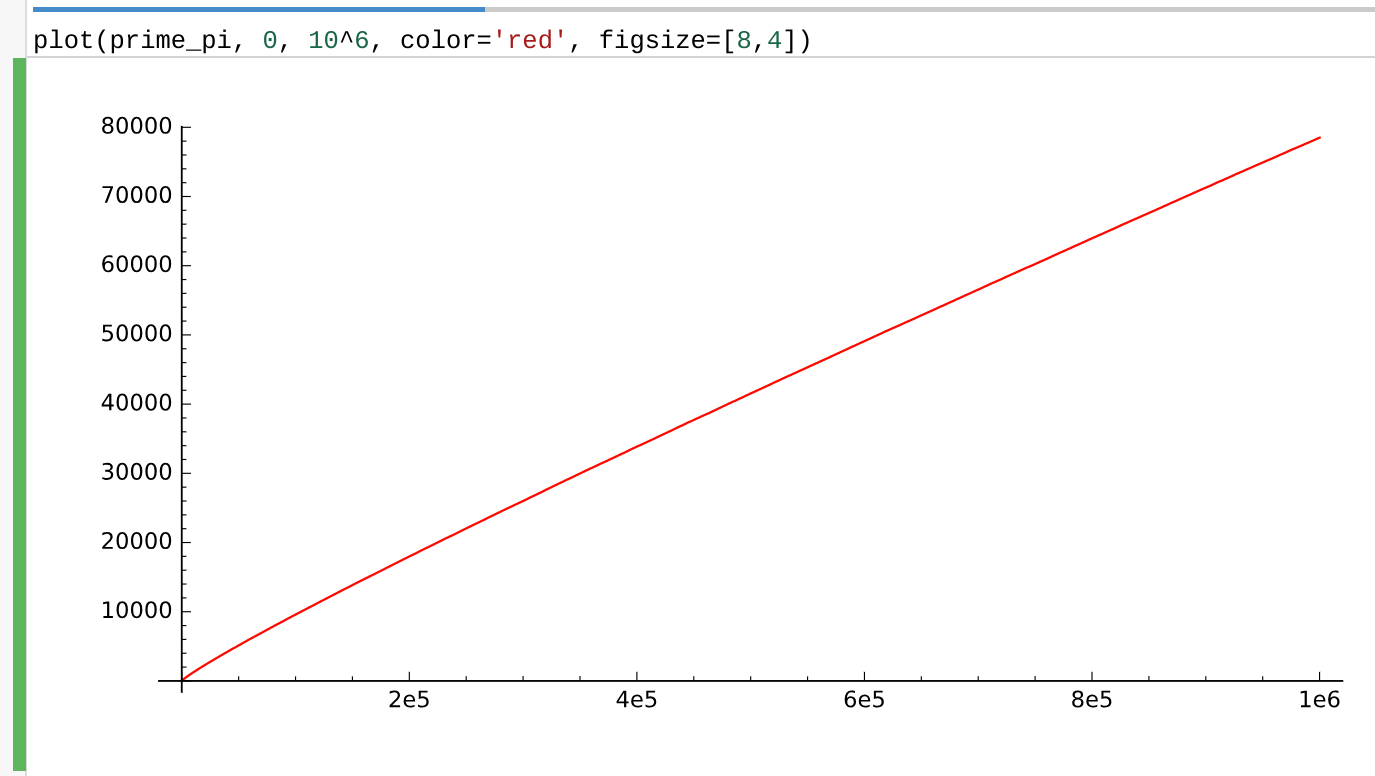
\includegraphics[width=.98\textwidth]{pics/prime-pi-1000000}

\end{frame}

\begin{frame}{Answer: The Riemann Hypothesis (first formulation)}
  \begin{block}{}
    The number of prime numbers less than $X$ is
    approximately $\Li(X)$ and this approximation is essentially square
    root accurate.
  \end{block}
  \begin{center}
    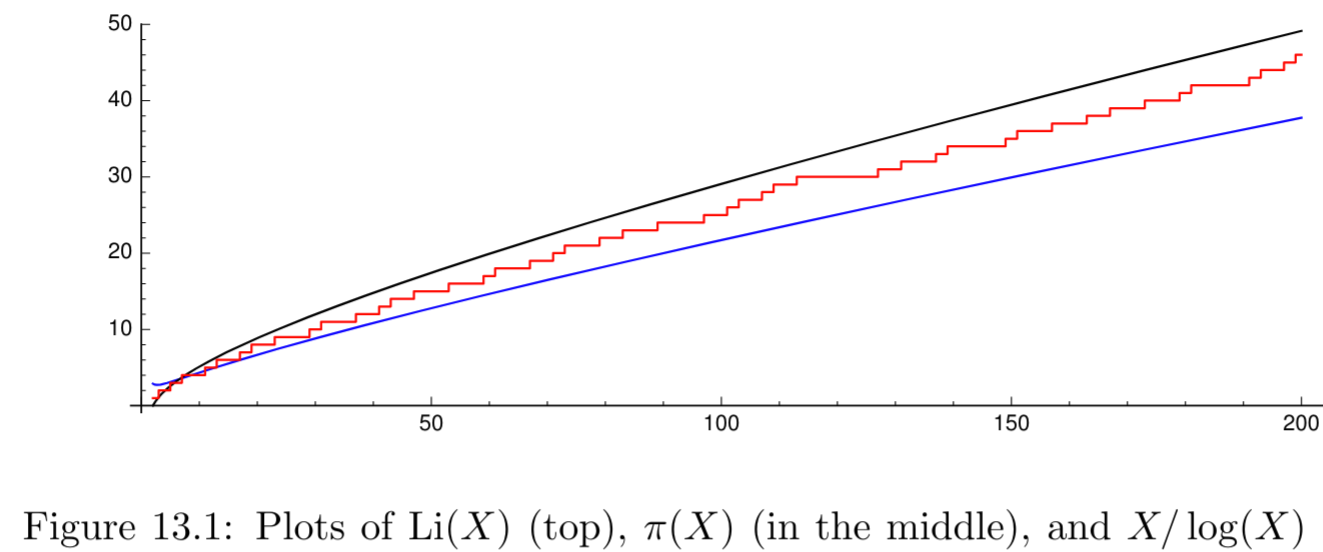
\includegraphics[width=.47\textwidth]{pics/plot-pi-Li}
    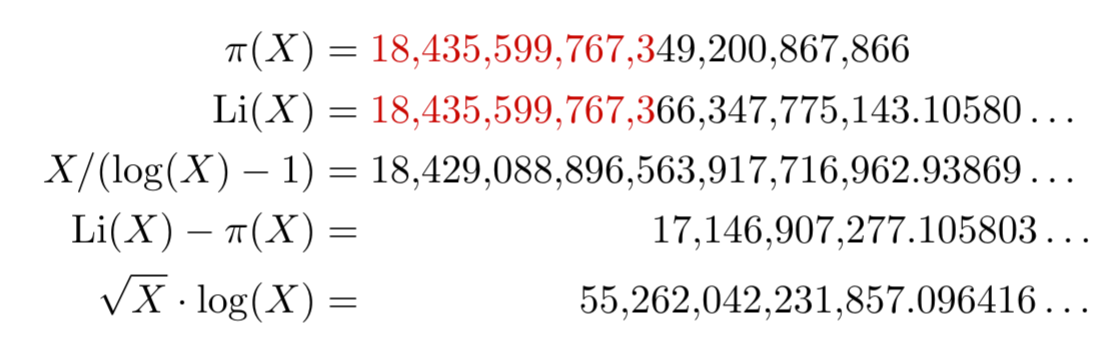
\includegraphics[width=.47\textwidth]{pics/ten24}
  \end{center}

$$
\pi(X) = \#\{\text{primes } \leq X\} \sim \Li(X) = \int_2^{X} \frac{1}{\log(t)} dt
$$

\end{frame}

\begin{frame}{Answer: The Riemann Hypothesis  (second formulation)}
  \begin{block}{}
    The prime power staircase $\psi(X)$ is essentially square root close
    to the 45 degree straight line.
  \end{block}

  $\psi(x)$: ``Our staircase starts on the ground at $x=0$ and the height of the
  riser of the step at $x=1$ will be $\log(2\pi)$. The height of the
  riser of the step at $x=p^n$ will not be $1$
  but rather: the step at $x=p^n$ will have the height of its riser
  equal to $\log p$.''

\begin{center}
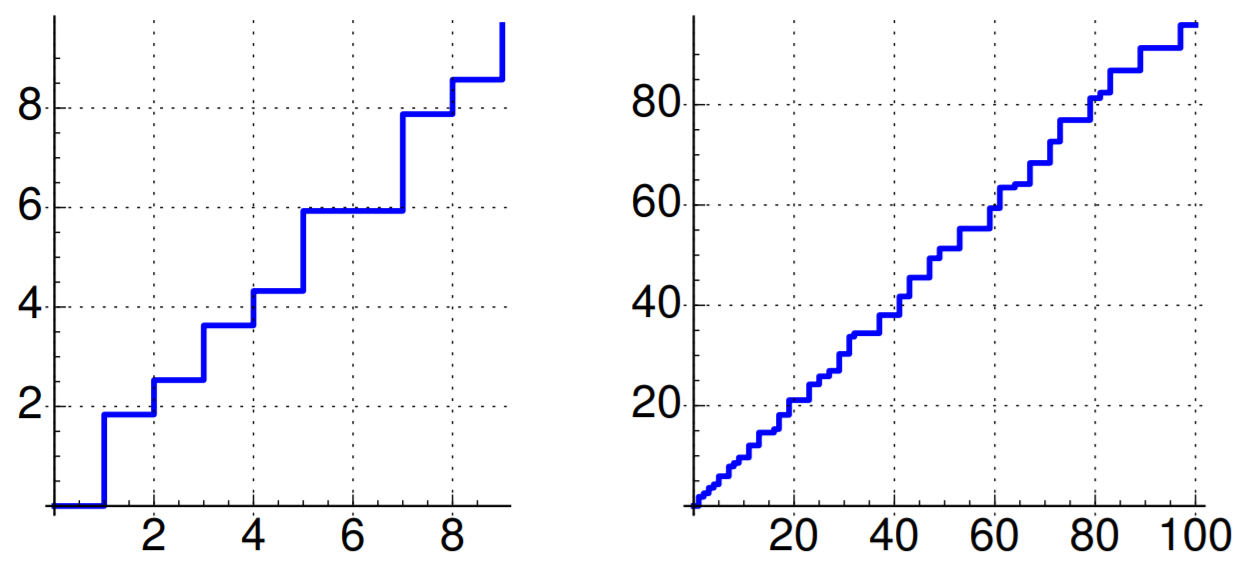
\includegraphics[height=.4\textheight]{pics/psi}
\end{center}
\end{frame}

\begin{frame}{Answer: The Riemann Hypothesis (third formulation)}
  \begin{block}{}
    The Fourier transform
    of the derivative of $\psi(X)$ \emph{``is basically''}
    a discrete distribution supported at the imaginary parts of the
    zeros of the Riemann Zeta function.

  \end{block}
\vfill

We deleted this formulation from the book, since it was too technical to state properly (it's the {\em explicit formula}).\footnote{After deleting this, we accidentally didn't relabel the ``fourth formulation", which confused readers.}

\vfill

Instead, we illustrate the heck out of it!

\vfill

\end{frame}

\begin{frame}{Fourier transform of $\Psi'(x)$ (just four terms!)}

    \begin{align*}
   f(t) =& -{\frac{\log(2)}{2^{1/2}}}\cos(t\log(2))- {\frac{\log(3)}{3^{1/2}}}\cos(t\log(3))\\
     &\qquad -{\frac{\log(2)}{4^{1/2}}}\cos(t\log(4))-{\frac{\log(5)}{5^{1/2}}}\cos(t\log(5))
  \end{align*}

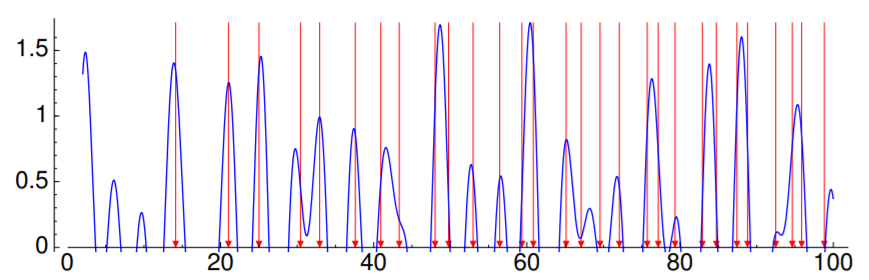
\includegraphics[height=.42\textheight]{pics/prime-power-freq-5}

\vfill

\begin{itemize}
\item Anybody can easily plot this.
\item Arrows point to imaginary parts of zeros of $\zeta(s)$!
\end{itemize}

\end{frame}



\begin{frame}{Fourier transform of $\Psi'(x)$ (first 20 terms)}


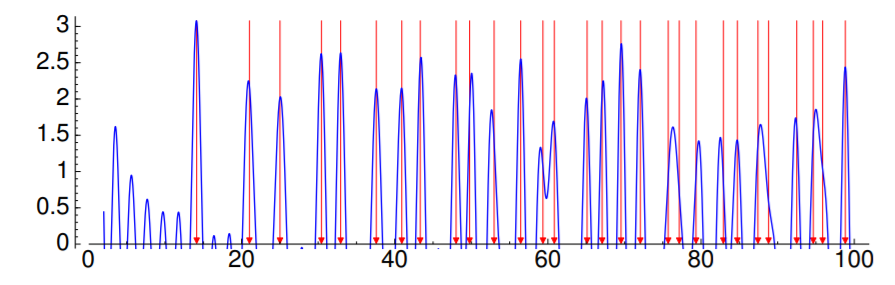
\includegraphics[height=.41\textheight]{pics/prime-power-freq-20}

\vfill

$$
-\sum_{p^n\leq 20}{\frac{\log(p)}{p^{n/2}}}\cos(t\log(p^n))
$$

\end{frame}


\begin{frame}{Fourier transform of $\Psi'(x)$ (first 500 terms)}

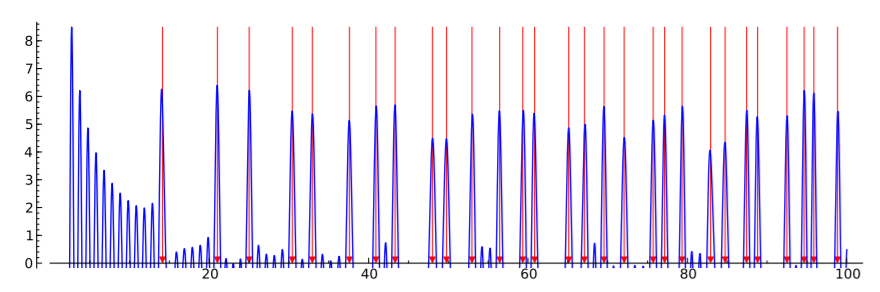
\includegraphics[height=.43\textheight]{pics/prime-power-freq-500}
\vfill

$$
-\sum_{p^n\leq 500}{\frac{\log(p)}{p^{n/2}}}\cos(t\log(p^n))
$$

{\bf Take this home:}
{\em The Fourier transform of the derivative of the prime power staircase ``is'' the
zeros of the Riemann zeta function.}

\end{frame}


\begin{frame}{It goes both ways!}

The Fourier transform of the zeros ``is'' prime powers:

\begin{center}
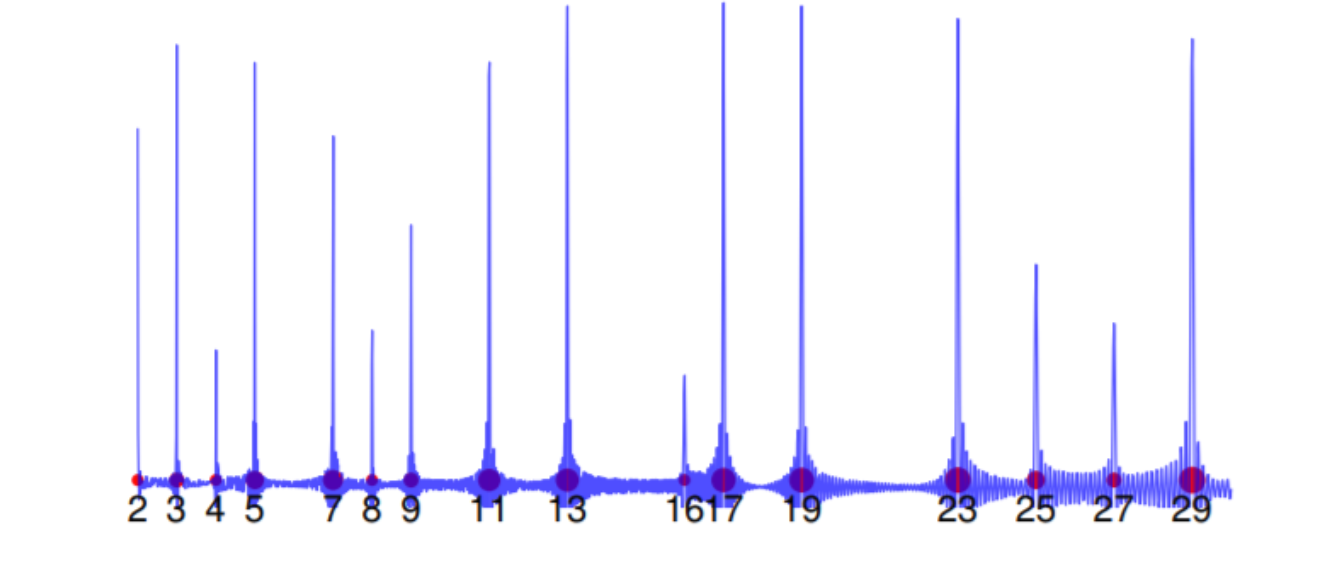
\includegraphics[height=.55\textheight]{pics/zeros-series-1000}
\end{center}

$$-\sum_{i=1}^{1000}
   \cos(\log(s)\theta_i)$$

%$\theta_1 \sim 14.13, \ldots$ are the
%   first $1000$ contributions to the imaginary parts
%   of zeros.

\end{frame}

\begin{frame}{Riemann untangled this to get $\pi(x)$...}

We finish book with manipulation to approximate $\pi(x)$
by a sum of smooth functions $R_k(x)$ involving the $\theta_i$.
\vfill

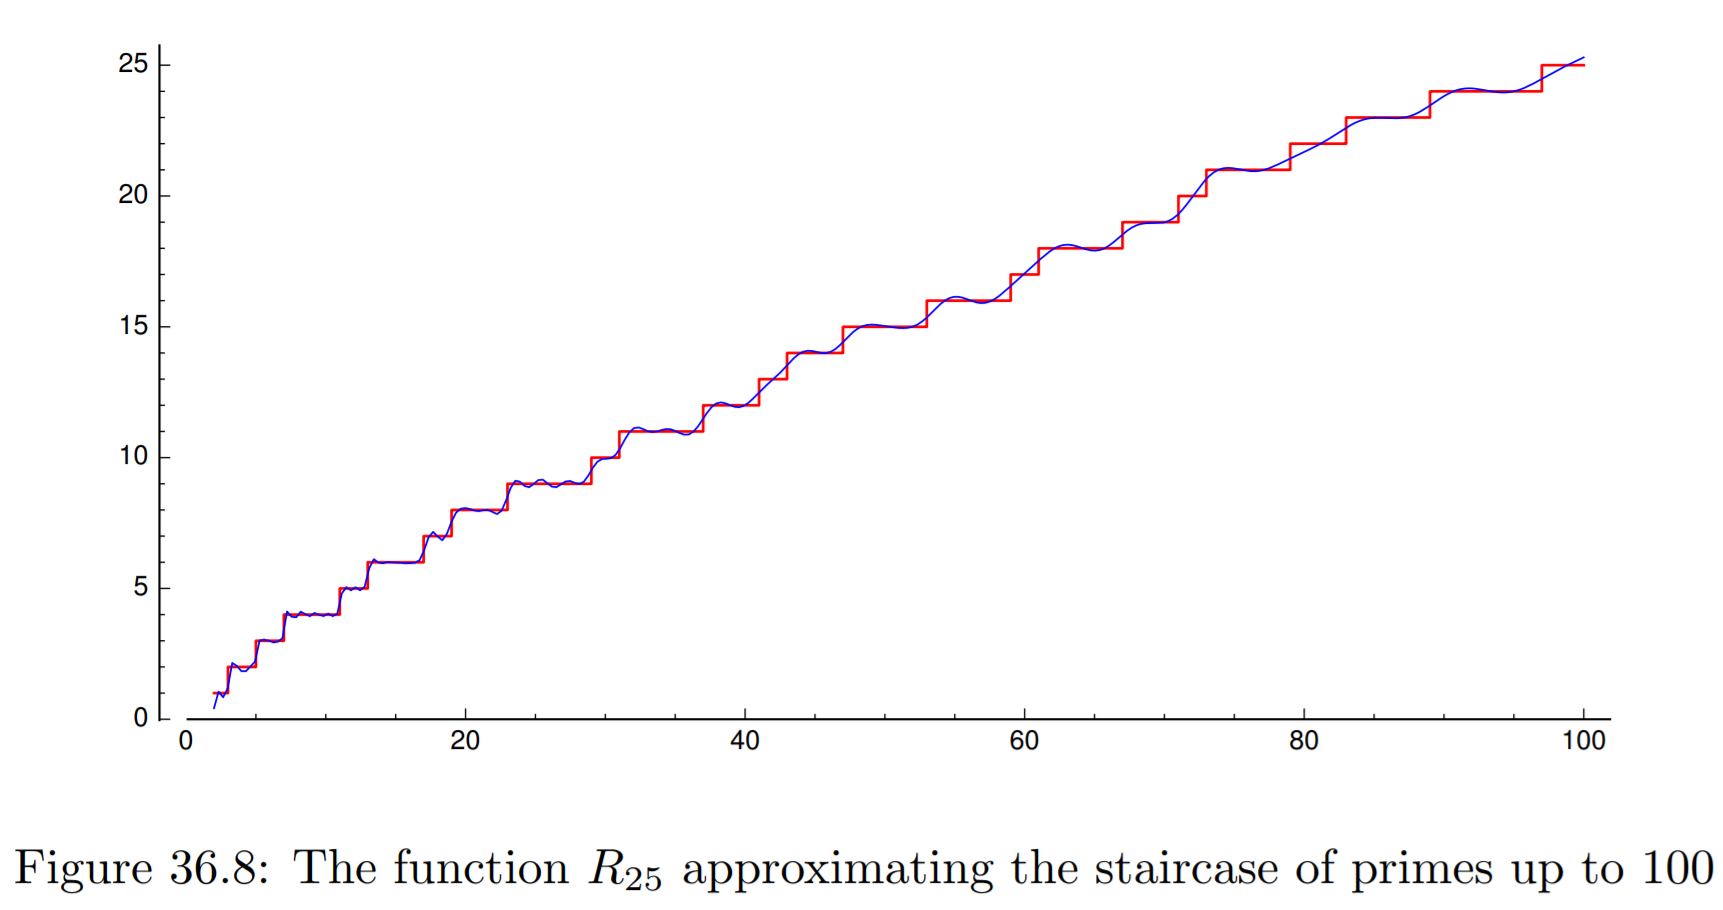
\includegraphics[height=.65\textheight]{pics/R25-approx}

\vfill
Inspiration: Zagier's lecture ``The First 50 million prime numbers''.
\end{frame}


\begin{frame}{$R_{50}$ approximates $\pi(x)$ very well!}

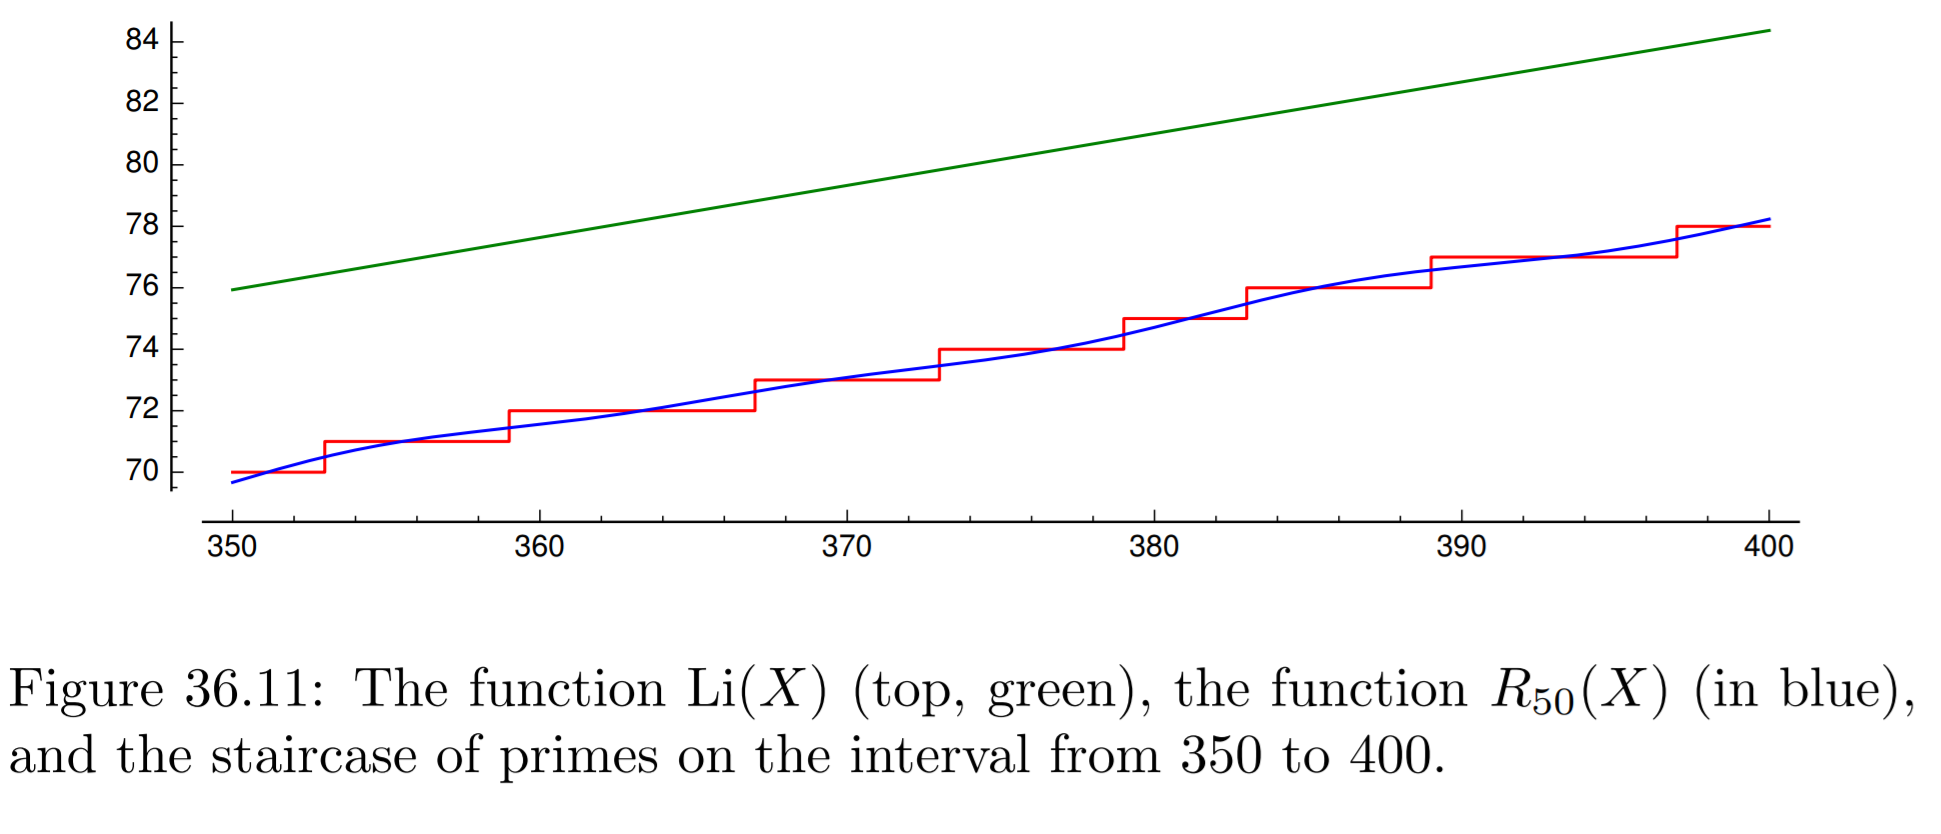
\includegraphics[height=.55\textheight]{pics/Li-R50-pi}

\end{frame}



\begin{frame}{Answer: The Riemann Hypothesis (fourth formulation)}
  \begin{block}{}
    All the nontrivial zeroes\index{nontrivial zeroes} of $\zeta(s)$ lie on the vertical
    line in the complex plane consisting of the
    complex numbers with real part equal to $1/2$.
  \end{block}
\end{frame}


\mysection{3}{Publishing a Book}

\begin{frame}{How to Publish the book:  Self publish!?}
\begin{block}{Self publishing?}
    Just put it on my website and see what happens.
          \begin{itemize}
            \item Some people read it...
            \item It didn't really get \textbf{significant traction}.
            \item There was still that key \textbf{missing quality} step.
          \end{itemize}
          \end{block}
          \vfill
Will Hearst convinced us to publish with a commercial publisher.
Maybe he was tired of printing out copies to give to people?
\end{frame}

\begin{frame}{Finding a publisher}
\begin{block}{Finding the right publisher for {\em this book}...}
  \begin{itemize}
  \item Barry and I have both published a few books with a couple of publishers, over the years.
    \item Talked to many editors (the JMM was \textbf{very} helpful!)
    \item Looked at reputation, similar books, and who followed up
    \item Balanced competing goals (e.g., price, quality, rights)
    \item Kaitlin from Cambridge University Press won for this.
  \end{itemize}
  \end{block}
\end{frame}
%todo: fullname of Kaitlin


\begin{frame}{Typos and Mistakes}
\begin{block}{Or, making the book easier for people to read}
  \begin{itemize}
    \item Dozens of people carefully read drafts of
          the book and provided incredibly useful feedback.
          \textbf{THANK YOU!!}
    \item The publisher had a copy editor read the book,
          and provided complementary feedback.
    \item Don't expect your publisher to catch the sort of
          mistakes a mathematician catches:
          \begin{center}
            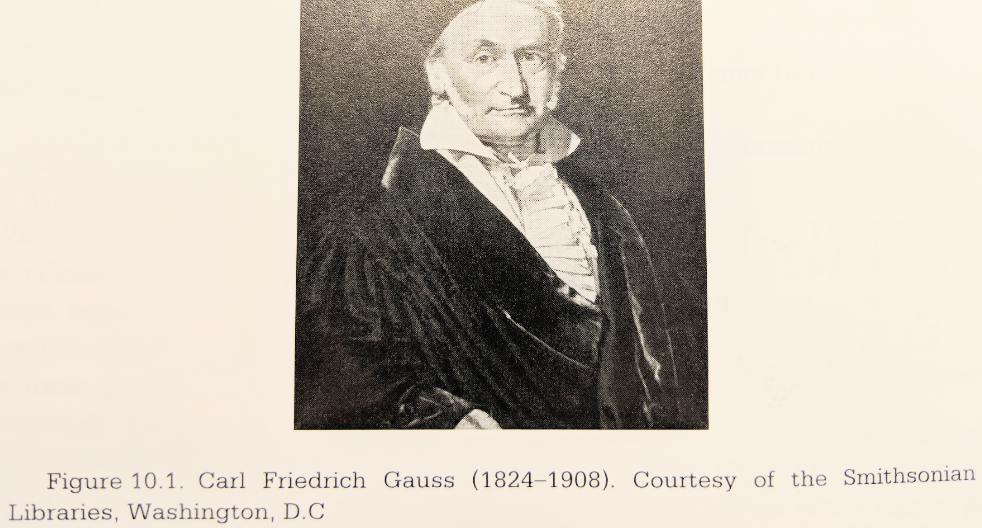
\includegraphics[height=.45\textheight]{pics/gauss}
          \end{center}
  \end{itemize}
  \end{block}
  % todo: better gauss picture
\end{frame}


\begin{frame}{Creating a Cover}


\begin{block}{Ideas for Components Included...}
  \begin{itemize}
    \item Title of book
    \item Our names
    \item Plot of $\zeta(s)$, using Sage's {\tt complex\_plot}
    \item Portrait of Riemann, the star of the book!
    \item Plots illustrating the main ideas of the book
    \item A ``classical'' look
  \end{itemize}
\end{block}

\vfill
There is a natural tension here: publisher vs author vs marketer

\end{frame}

\begin{frame}{What We Created}
  \begin{center}
    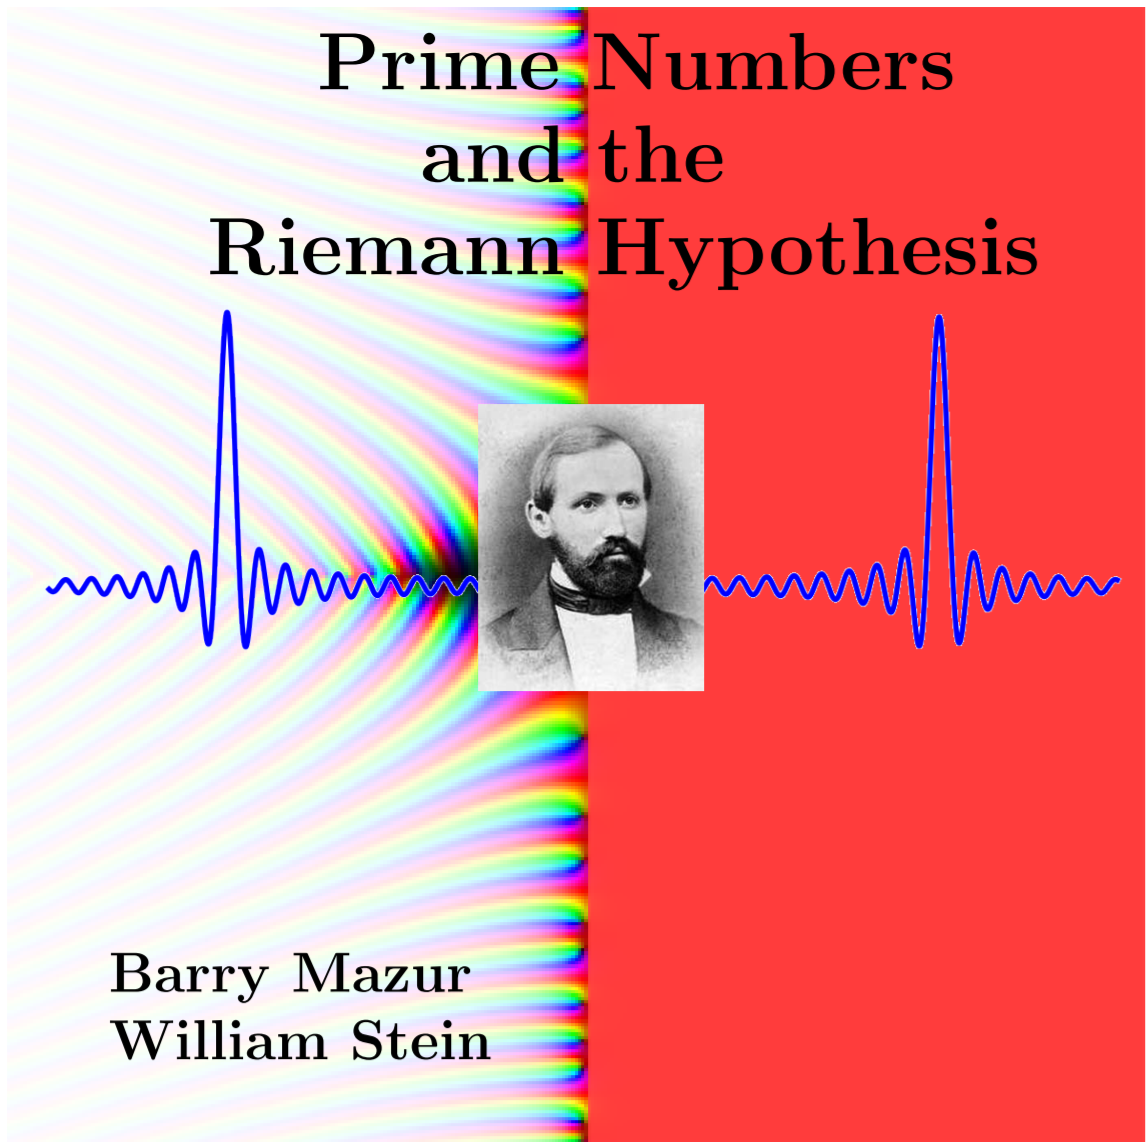
\includegraphics[height=.82\textheight]{pics/cover-we-wanted}
  \end{center}
\end{frame}

\begin{frame}{The Actual Cover}
% TODO: better quality!
  \begin{center}
    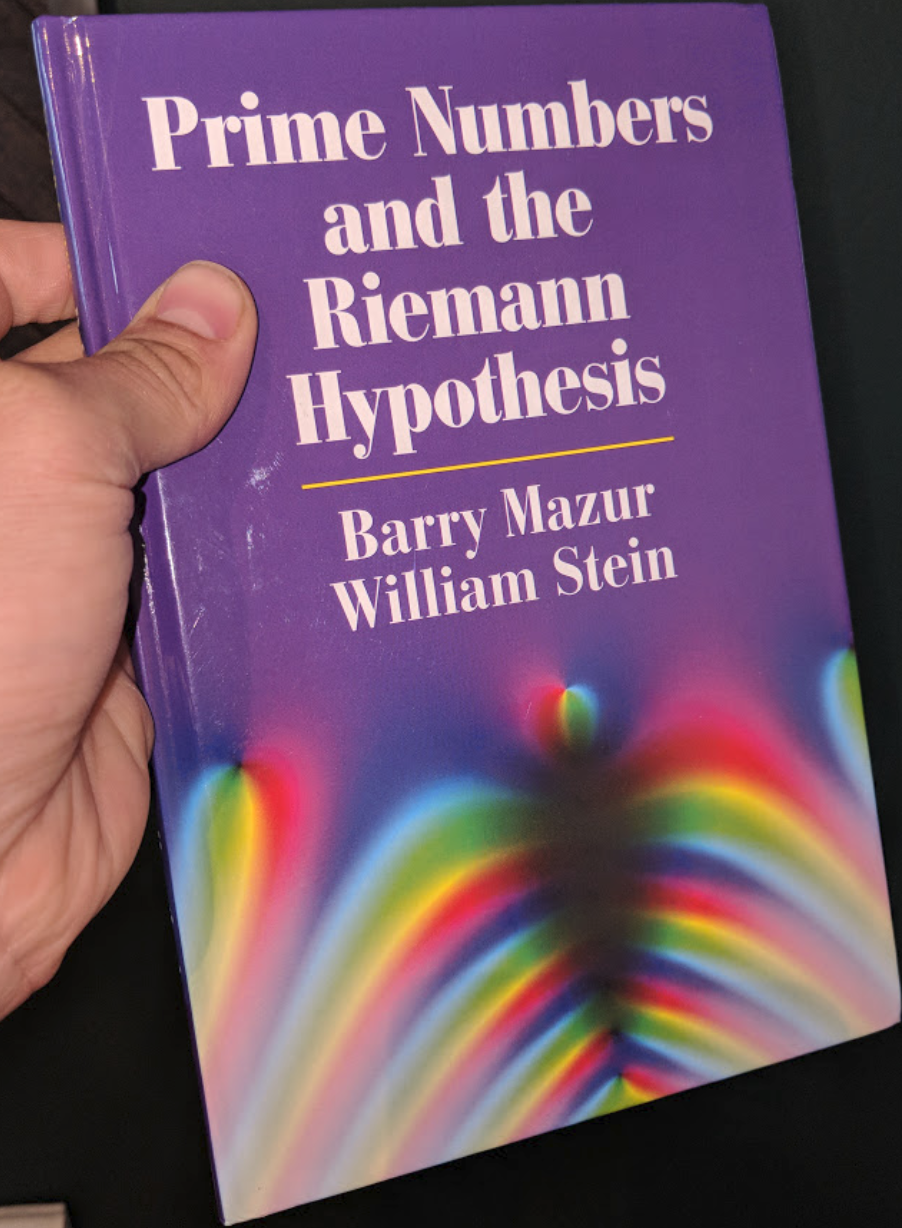
\includegraphics[height=.82\textheight]{pics/cover-front}
  \end{center}
\end{frame}

\begin{frame}{Endorsements for the back cover}
% TODO: better quality!
Will Hearst and John Cremona kindly wrote about our book...

  \begin{center}
    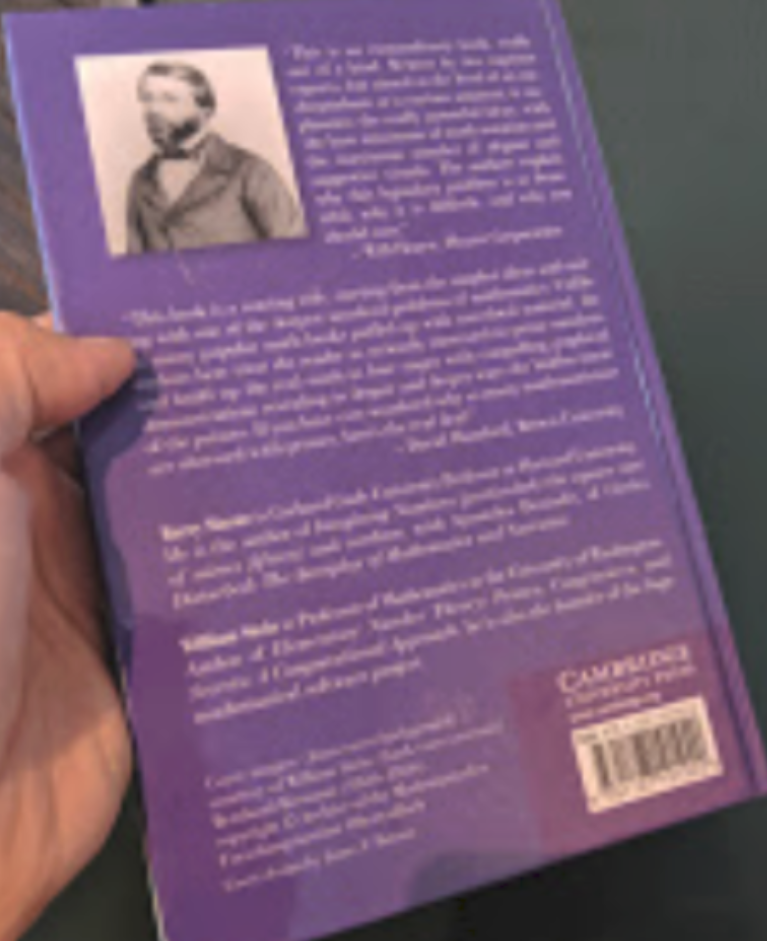
\includegraphics[height=.7\textheight]{pics/cover-back}
  \end{center}
\end{frame}

\begin{frame}{Production}
\begin{block}{Producing the book}
  \begin{itemize}
  \item Initial friction with production, e.g., ``Please provide Microsoft Word document.''
    \item Evidently, Cambridge Univ Press might have made some new positive steps toward better \LaTeX{} support.
    \item Some unfortunate physical issues with the very first printing.
    \item CUP strongly supported and marketed the book.
    \item Working with CUP has been a {\em very positive experience} overall.
  \end{itemize}
\end{block}
\end{frame}

\begin{frame}{Published!}

  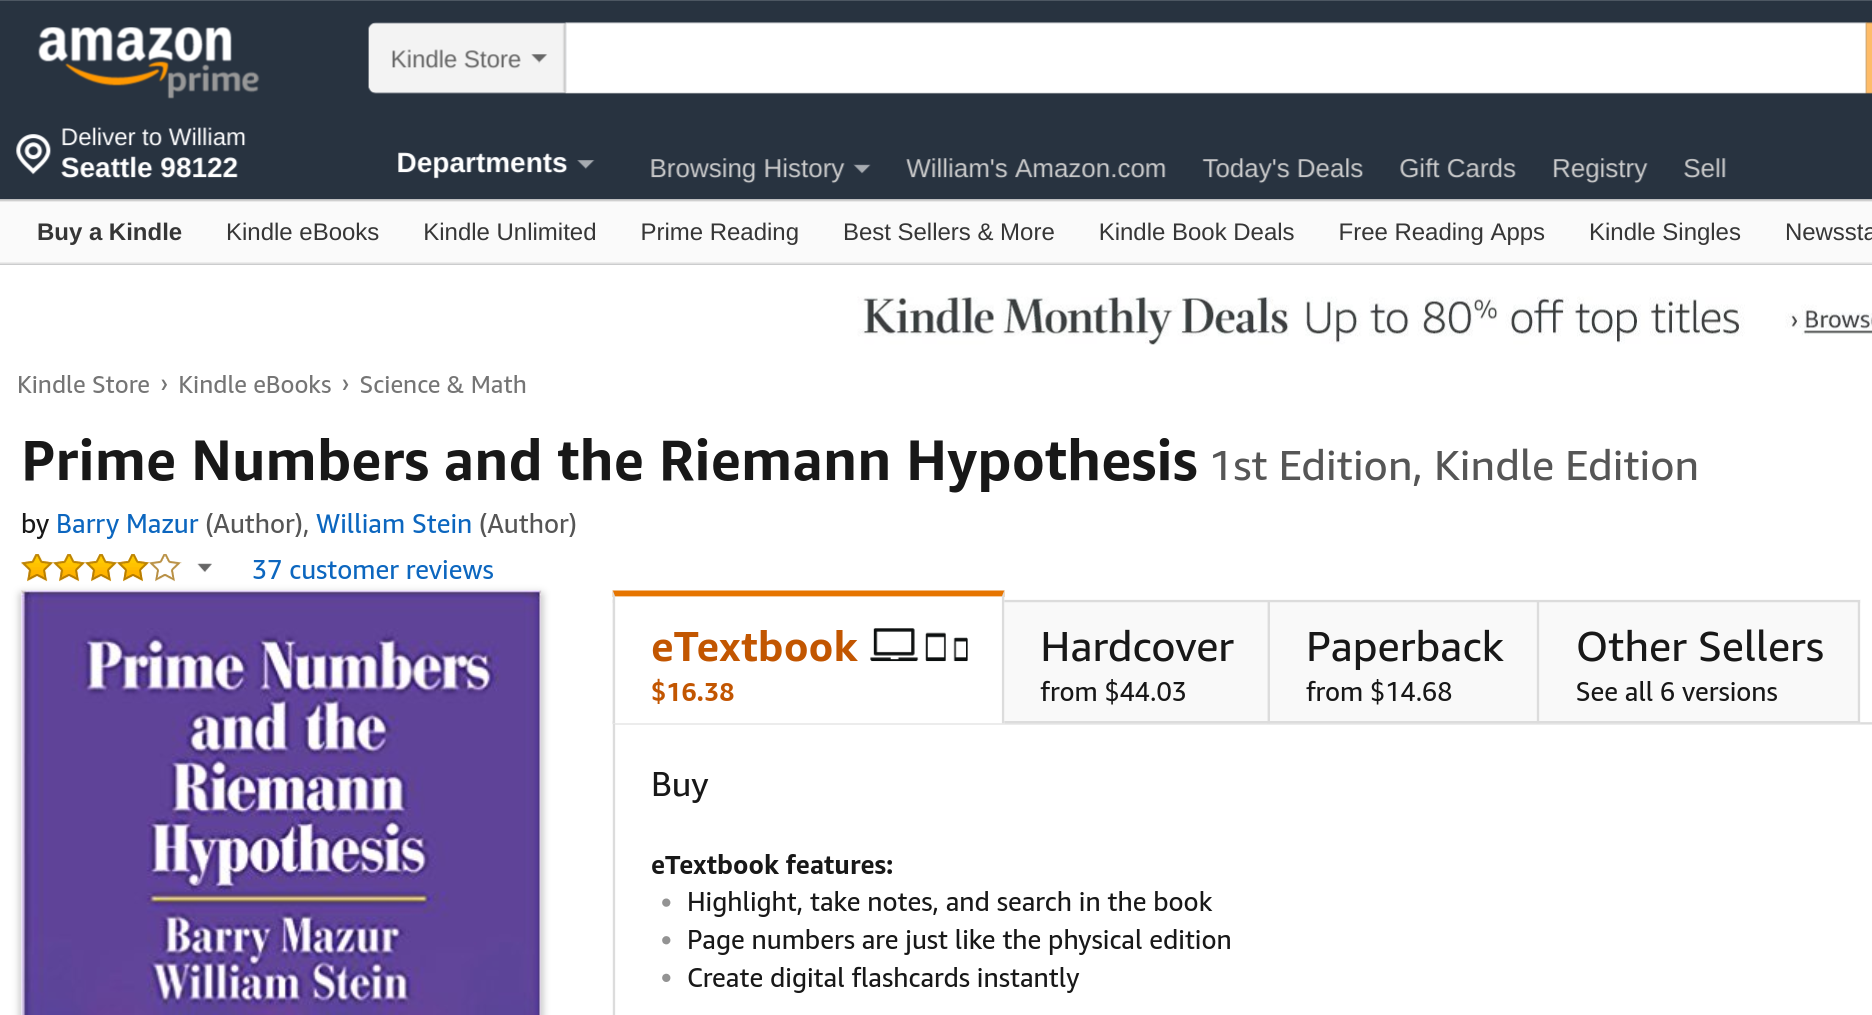
\includegraphics[width=.98\textwidth]{pics/amazon-prime}

\end{frame}



\begin{frame}{Reviews by Readers}

  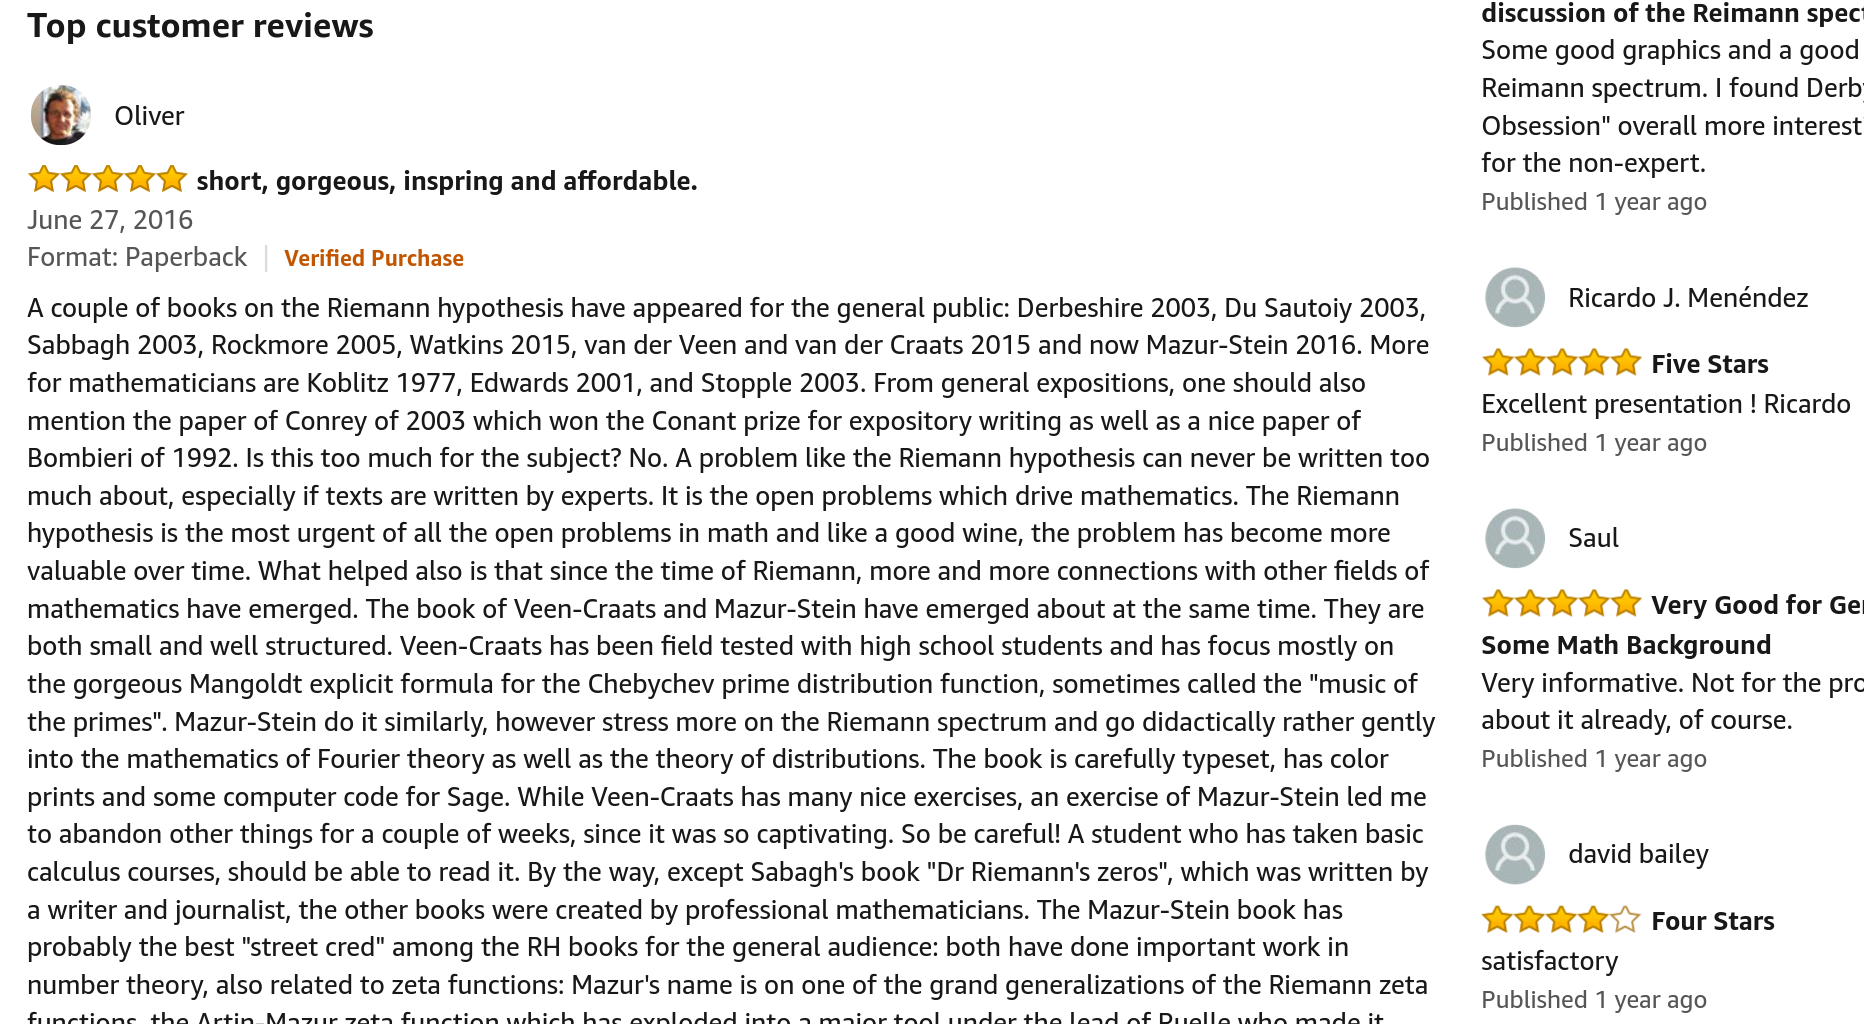
\includegraphics[width=.95\textwidth]{pics/amazon-review}

\hrulefill

  \vfill

  Negative reviews  mainly due to \textit{production issues},
  both with the physical book
  and the Kindle edition, which CUP fully addressed.

\end{frame}

\begin{frame}{Reception by Readers}
%todo: put in stuff here
  \begin{itemize}
    \item Sarnak's review in Bulletins
    \item Ash's review in ???
    \item Other reviews?  Granville?
    \item Prizes
  \end{itemize}
\end{frame}

\begin{frame}{Royalties}

  We sold some copies, so Cambridge University Press sent us some money.
  I'm spending my share on expenses for my dream dog:

  \begin{center}
    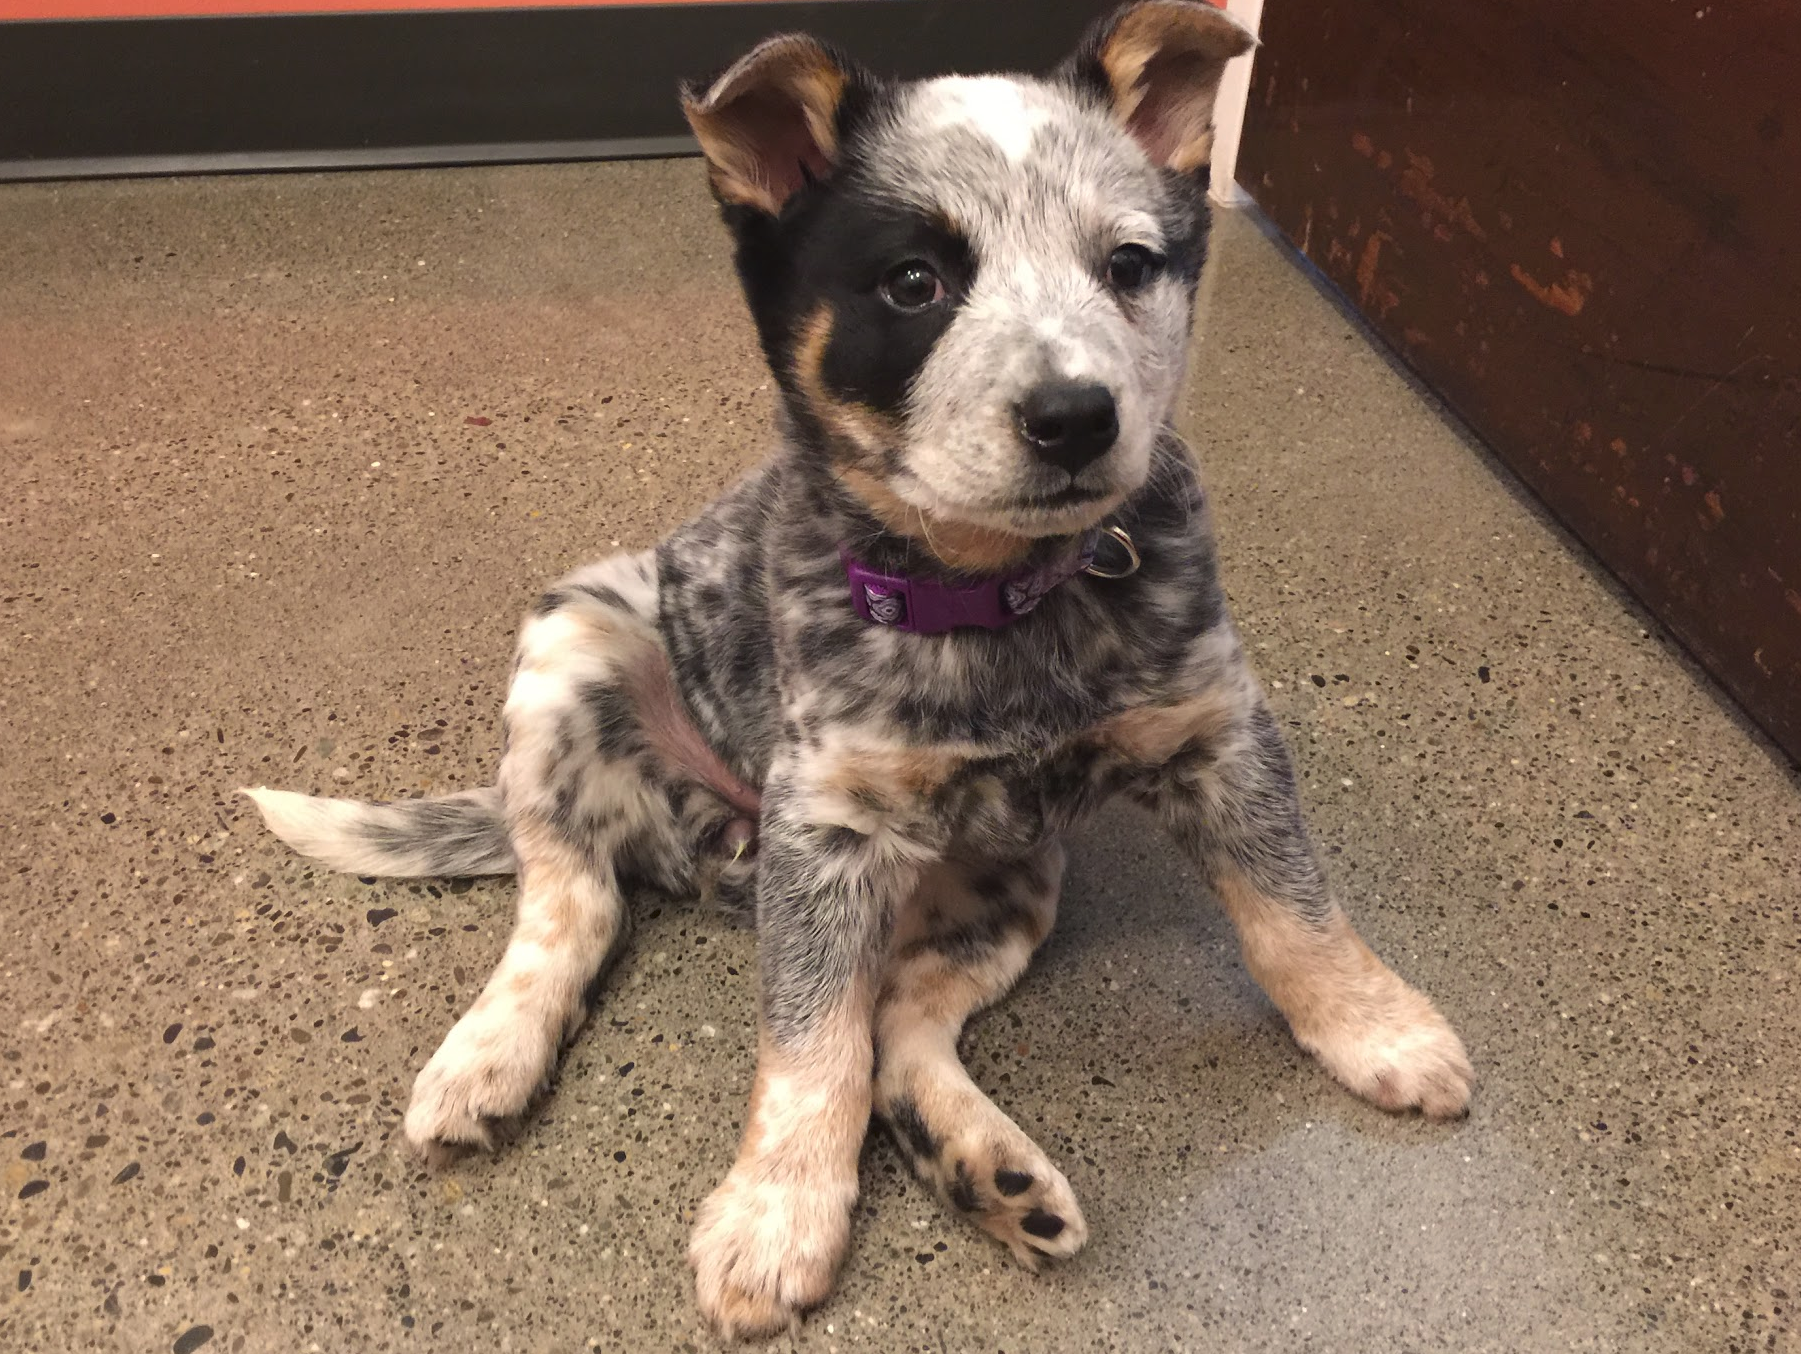
\includegraphics[height=.7\textheight]{pics/bella-puppy}
  \end{center}


\end{frame}


\begin{frame}[fragile]
  \frametitle{Translations}
  \begin{verbatim}
Dear Professor Stein,

Prime Numbers and the Riemann Hypothesis

I am delighted to inform you that we are currently
concluding an agreement with Nippon Hyoron Sha for
a Japanese language edition of your book. They plan
to print an edition of 2,500 copies initially, which
will be sold at approximately 2,200 JPY per copy.
  \end{verbatim}

  What to expect?
  \begin{itemize}
    \item  Also Korean?
    \item  Will they bother with French, etc.?
  \end{itemize}
\end{frame}


\begin{frame}
  \frametitle{Future plans}
  \begin{block}{Someday we hope to...}
  \begin{itemize}
    \item Create online fully interactive version of all the
    plots, which don't require knowing Sage to use.
    \item Finish related research on $L$-series of elliptic curves, connecting the rank to statistical
behavior of the $a_p$.
  \end{itemize}
  \end{block}
\end{frame}


\end{document}